\documentclass[ignorenonframetext,aspectratio=129]{beamer}
\setbeamertemplate{caption}[numbered]
\setbeamertemplate{caption label separator}{: }
\setbeamercolor{caption name}{fg=normal text.fg}
\beamertemplatenavigationsymbolsempty
\usepackage{lmodern}
\usepackage{amssymb,amsmath}
\usepackage{ifxetex,ifluatex}
\usepackage{fixltx2e} % provides \textsubscript
\ifnum 0\ifxetex 1\fi\ifluatex 1\fi=0 % if pdftex
  \usepackage[T1]{fontenc}
  \usepackage[utf8]{inputenc}
\else % if luatex or xelatex
  \ifxetex
    \usepackage{mathspec}
  \else
    \usepackage{fontspec}
  \fi
  \defaultfontfeatures{Ligatures=TeX,Scale=MatchLowercase}
\fi
\usetheme[]{BricksTemplate}
% use upquote if available, for straight quotes in verbatim environments
\IfFileExists{upquote.sty}{\usepackage{upquote}}{}
% use microtype if available
\IfFileExists{microtype.sty}{%
\usepackage{microtype}
\UseMicrotypeSet[protrusion]{basicmath} % disable protrusion for tt fonts
}{}
\newif\ifbibliography
\hypersetup{
            pdftitle={Galaxy-Bricks},
            pdfborder={0 0 0},
            breaklinks=true}
\urlstyle{same}  % don't use monospace font for urls
\usepackage{graphicx,grffile}
\makeatletter
\def\maxwidth{\ifdim\Gin@nat@width>\linewidth\linewidth\else\Gin@nat@width\fi}
\def\maxheight{\ifdim\Gin@nat@height>\textheight0.8\textheight\else\Gin@nat@height\fi}
\makeatother
% Scale images if necessary, so that they will not overflow the page
% margins by default, and it is still possible to overwrite the defaults
% using explicit options in \includegraphics[width, height, ...]{}
\setkeys{Gin}{width=\maxwidth,height=\maxheight,keepaspectratio}

% Prevent slide breaks in the middle of a paragraph:
\widowpenalties 1 10000
\raggedbottom

\AtBeginPart{
  \let\insertpartnumber\relax
  \let\partname\relax
  \frame{\partpage}
}
\AtBeginSection{
  \ifbibliography
  \else
    \let\insertsectionnumber\relax
    \let\sectionname\relax
    \frame{\sectionpage}
  \fi
}
\AtBeginSubsection{
  \let\insertsubsectionnumber\relax
  \let\subsectionname\relax
  \frame{\subsectionpage}
}

\setlength{\parindent}{0pt}
\setlength{\parskip}{6pt plus 2pt minus 1pt}
\setlength{\emergencystretch}{3em}  % prevent overfull lines
\providecommand{\tightlist}{%
  \setlength{\itemsep}{0pt}\setlength{\parskip}{0pt}}
\setcounter{secnumdepth}{0}
\usepackage{titling}

\pretitle{%
  \begin{center}
  \LARGE
  
\includegraphics[width=4cm,height=6cm]{logo.png}\\[\bigskipamount]
}
\posttitle{\end{center}}

\title{Galaxy-Bricks}
\subtitle{Vers une plateforme d'analyse de données collaborative}
\author{Simon Bénateau\(^1\), Sébastien Turpin\(^1\), Yvan Le
Bras\(^2\)\\[2\baselineskip]Muséum National d'Histoire Naturelle\\
1. UMR Centre d'Ecologie et des Sciences de la COnservation\\
2. UMS PATRImoine NATurel}
\date{15 mai 2019}

\begin{document}
\frame{\titlepage}

\begin{frame}{Vigie nature}

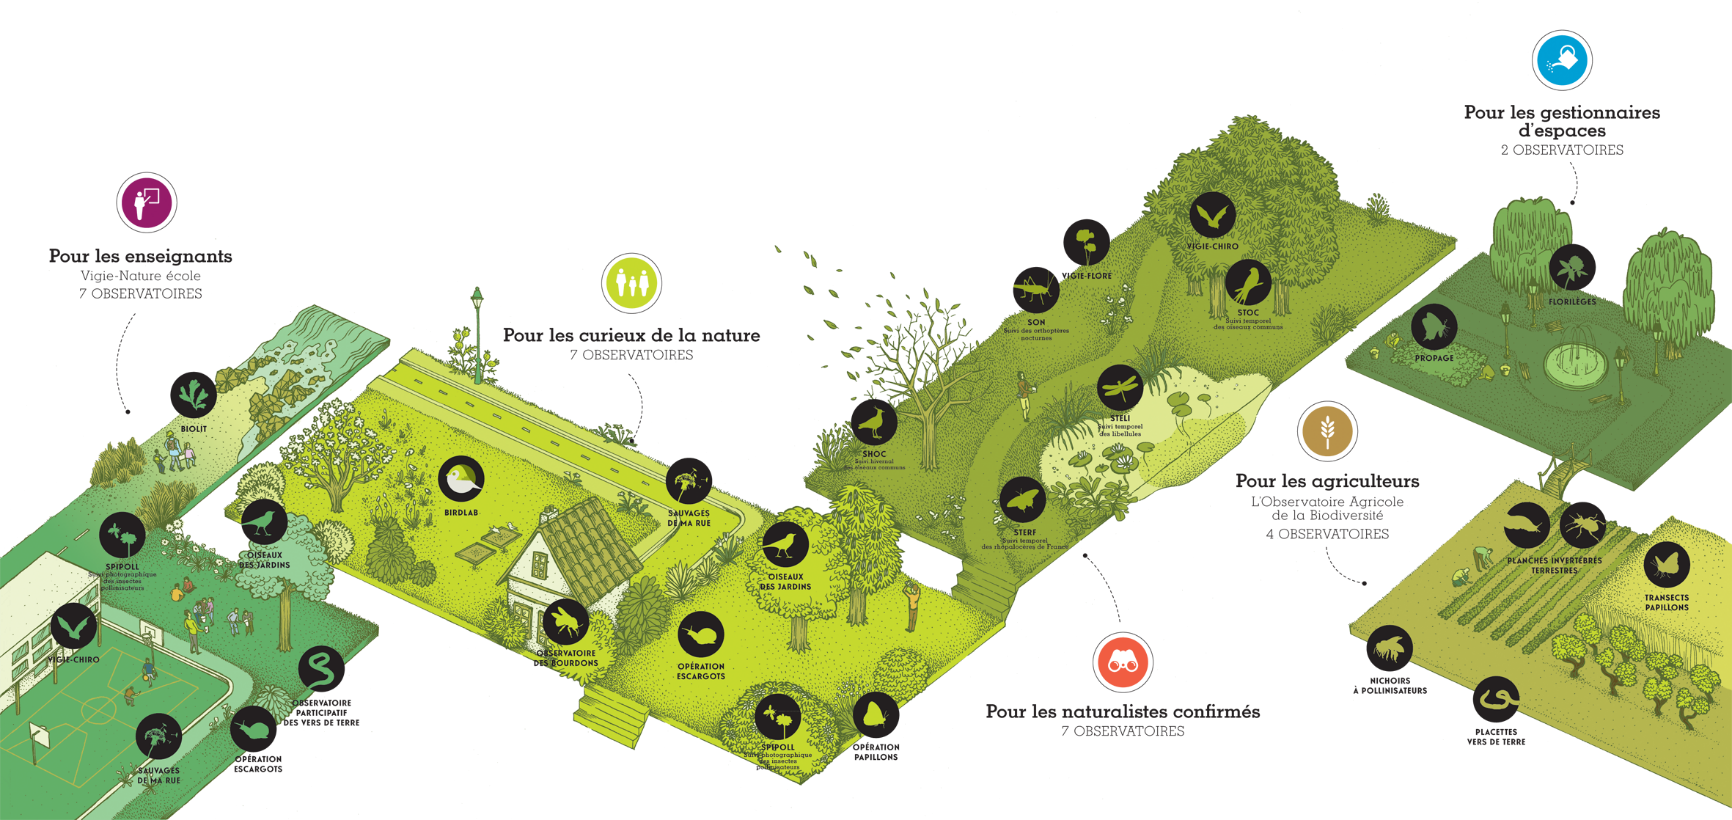
\includegraphics{figures/observatoires_vigienature_aml.jpg} - bulle
-\textgreater{} clarifier -\textgreater{} regarder slide Karine

\end{frame}

\begin{frame}{Organisation du réseau d'acteurs}

\includegraphics{figures/Vigie-Nature-Network.jpg} - clair sur les
boites

\end{frame}

\begin{frame}{Destination des plateformes d'analyse de données}

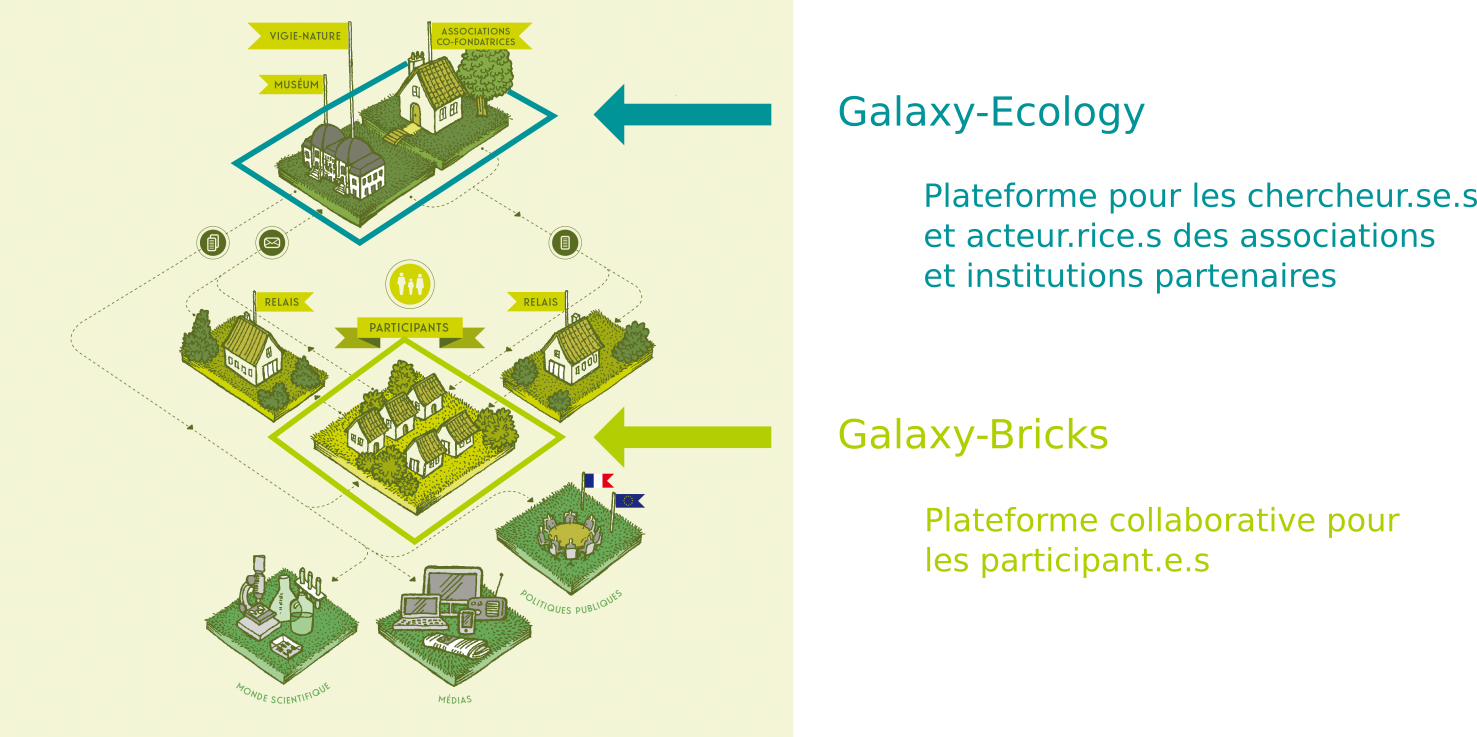
\includegraphics{figures/Vigie-Nature-Network-fr.png} - Bien mais à voir
pour clarifier

\end{frame}

\begin{frame}{Objectifs identifiés - ``grand public''}

\begin{itemize}
\tightlist
\item
  Proposer de nouvelles possibilités pour la participation citoyenne
\item
  Donner un accès aux données et permettre leur exploitation
\item
  Donner aux participants les moyens de répondre aux questions qu'ils se
  posent sur les données
\end{itemize}

\end{frame}

\begin{frame}{Objectifs identifiés - Vigie Nature Ecole}

\begin{itemize}
\tightlist
\item
  Proposer un nouvel outil pour l'apprentissage de la démarche
  scientifque
\item
  Formation à l'analyse de données
\item
  Possibilité de proposer une approche interdiciplinaire
\end{itemize}

\end{frame}

\begin{frame}{Réflexion sur l'ergonomie}

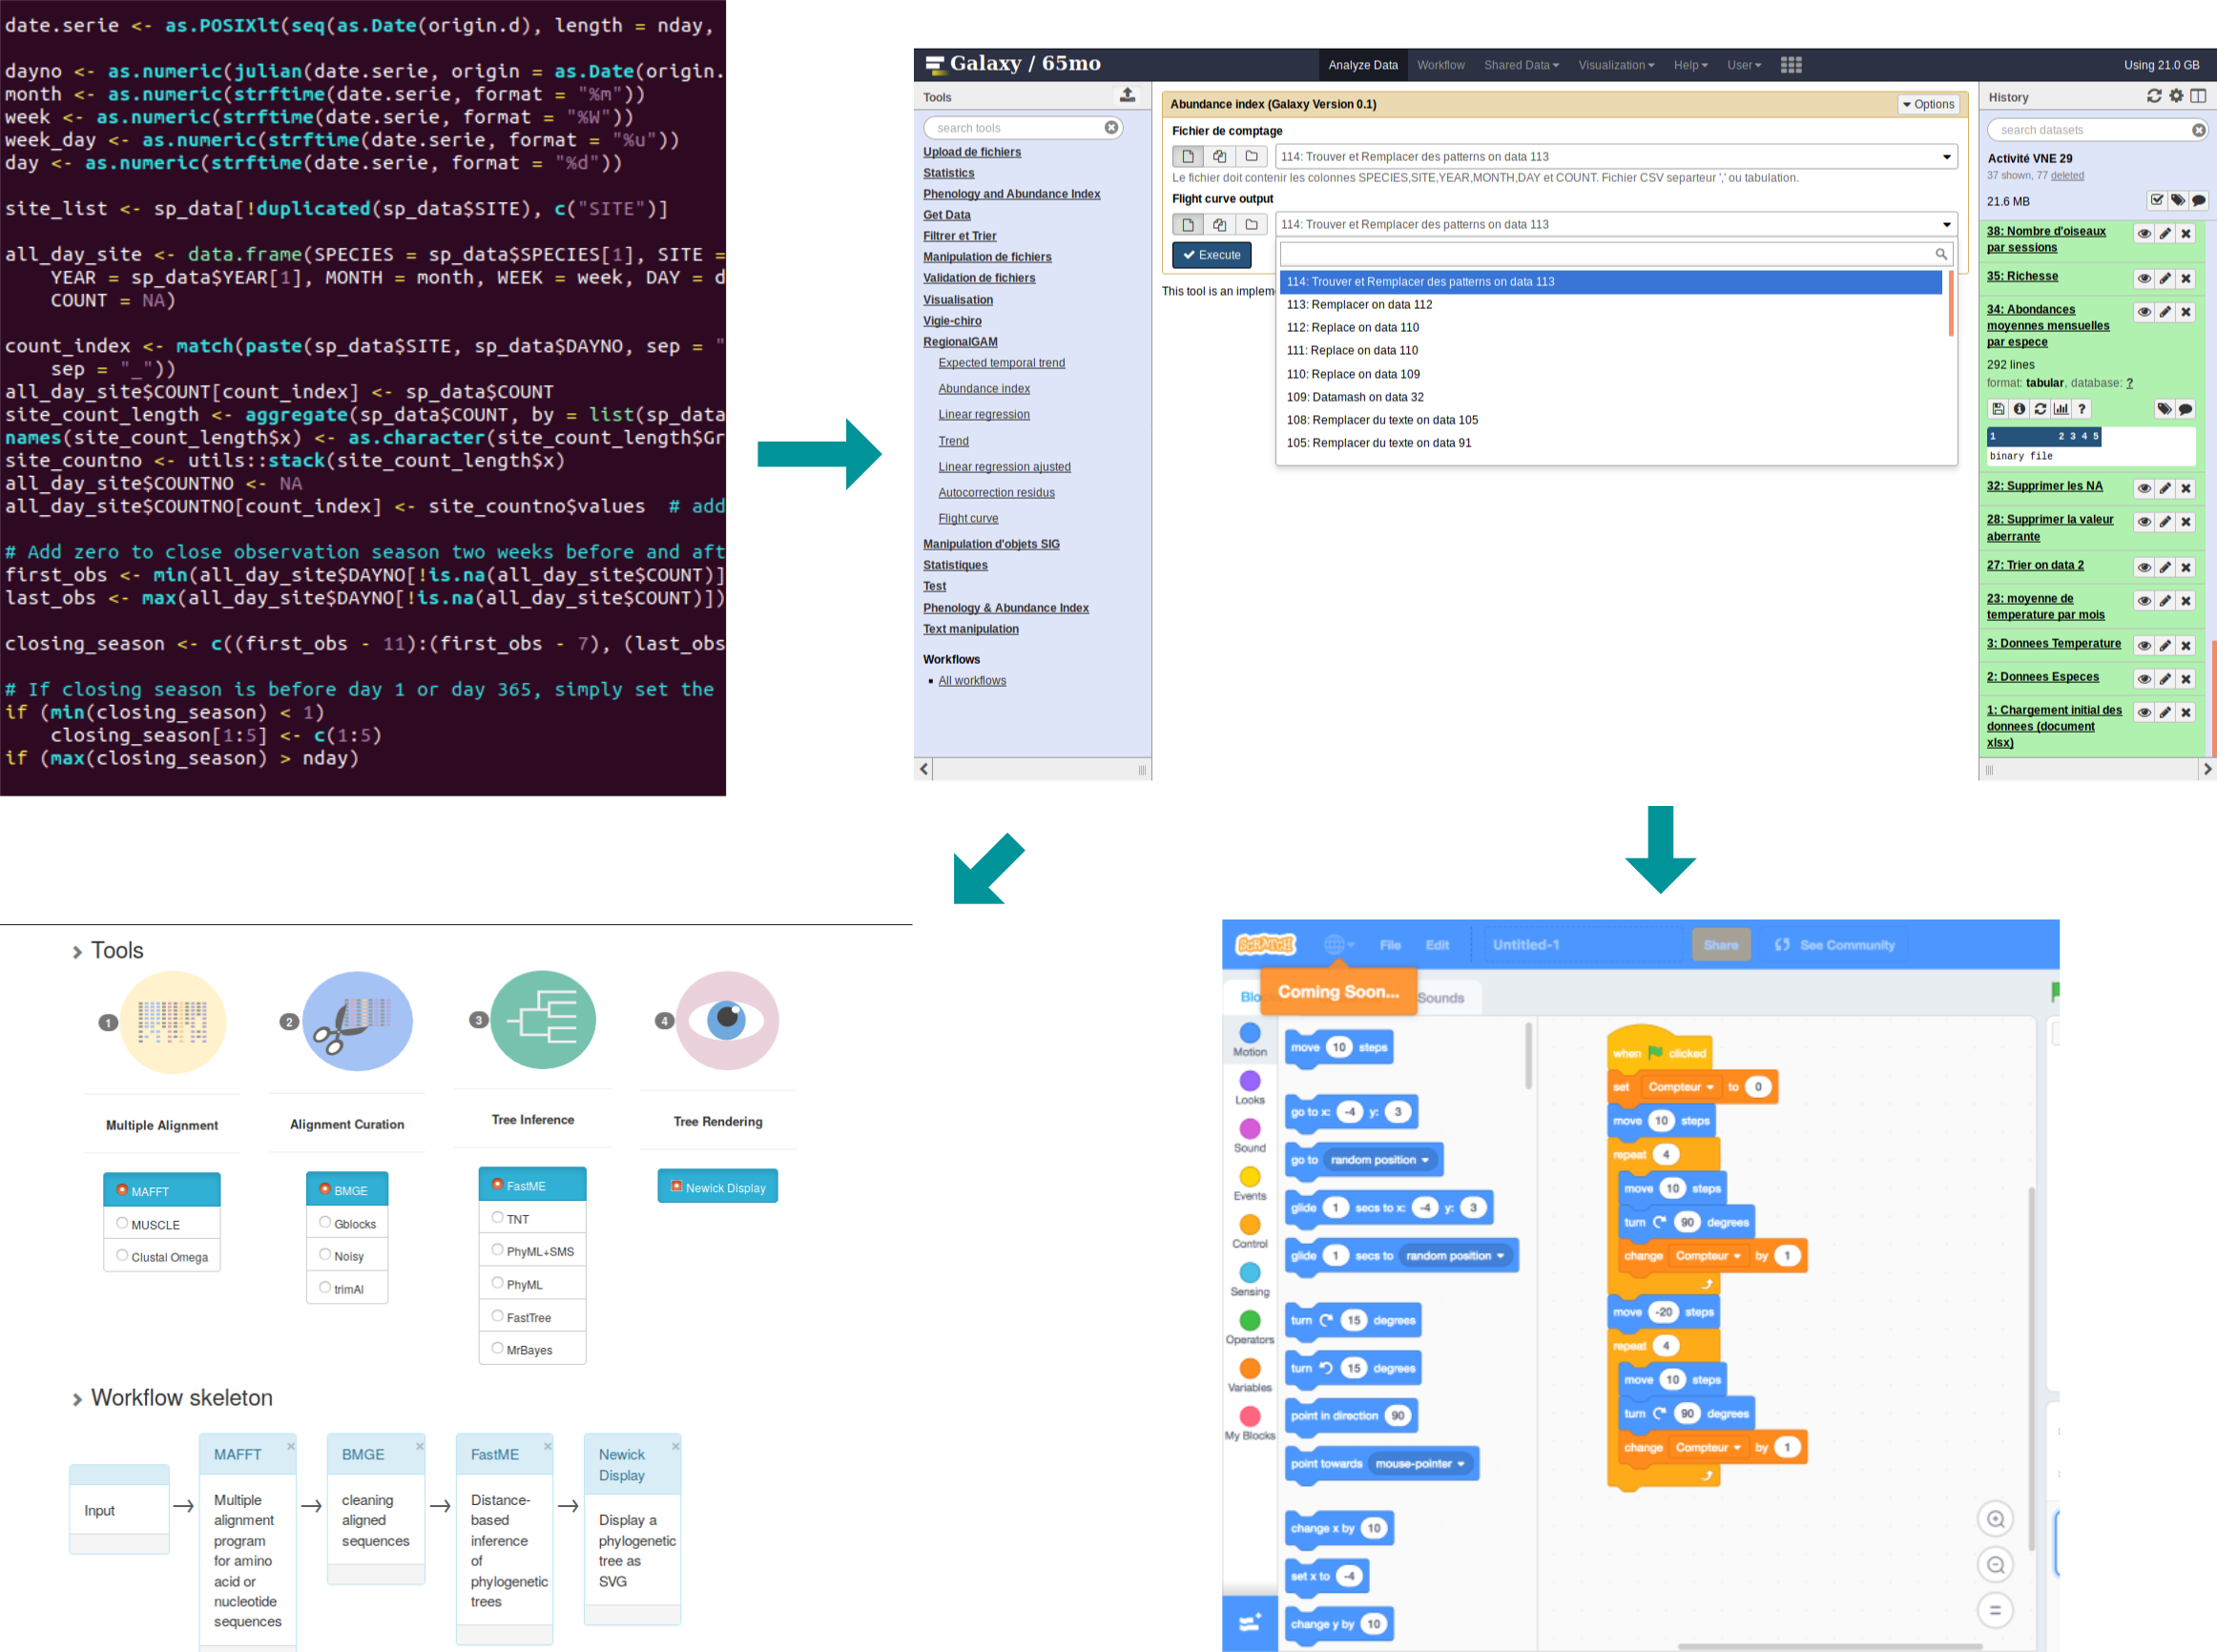
\includegraphics{figures/codeToTool.png}

\end{frame}

\begin{frame}{Nécessité de formation}

\begin{itemize}
\tightlist
\item
  Formation à l'outil via des tutoriels
\item
  Formation à l'analyse de données écologiques contextualisée
\item
  Création de supports interactifs
\end{itemize}

\end{frame}

\begin{frame}{Possibilité de partage}

\begin{block}{Au sein de Galaxy}

\begin{itemize}
\tightlist
\item
  Données
\item
  Outils
\item
  Workflow
\item
  Résultats
\item
  Rapports
\end{itemize}

\end{block}

\begin{block}{Plateforme d'échange}

\begin{itemize}
\tightlist
\item
  Forum
\item
  Chat
\end{itemize}

\end{block}

\end{frame}

\begin{frame}{Perspectives}

\begin{itemize}
\tightlist
\item
  Analyse collaborative
\end{itemize}

\end{frame}

\begin{frame}{Merci}

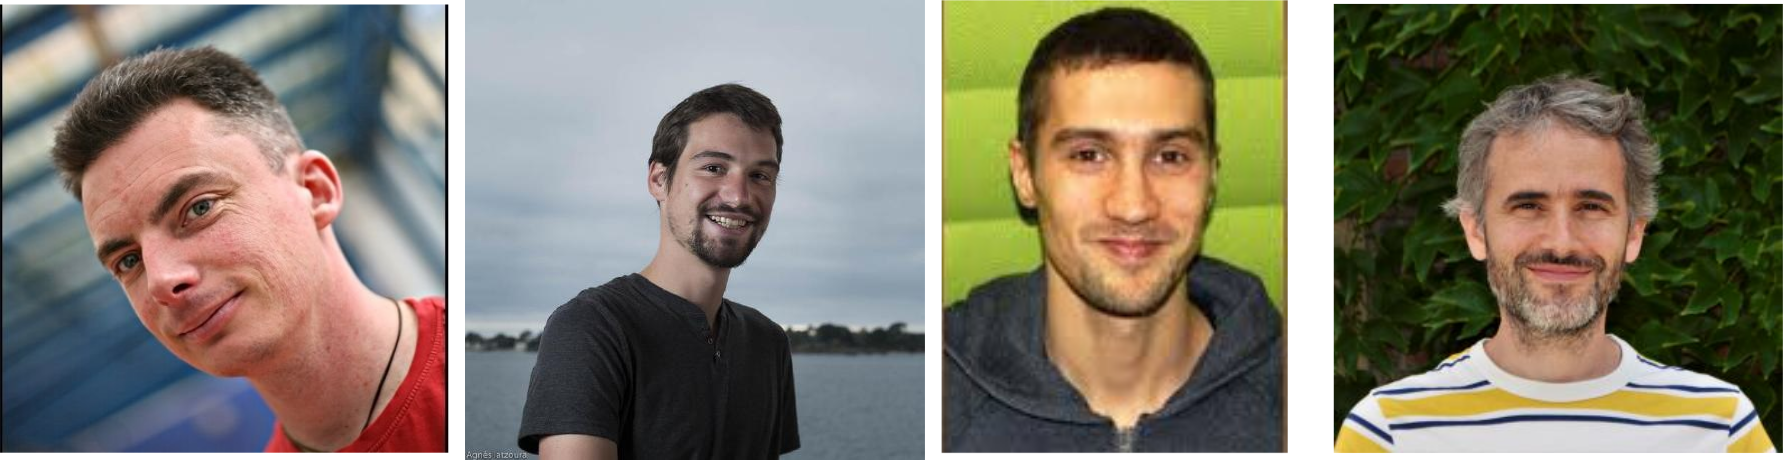
\includegraphics{figures/team.png.png}

\end{frame}

\end{document}
